% Kompilieren mit: pdflatex -shell-escape uebung
\documentclass{uebblatt}

\newcommand{\refaufgabe}[1]{#1} % TODO: wir sollten irgendwie Übungsaufgaben (vom ersten Blatt) mit Namen referenzieren, nicht per Nummer. Also wie mit \ref in LaTeX.
% Wir können die Blätter auch einfach zusammenlegen.
% Dann mit \refstepcounter arbeiten.

\begin{document}

\maketitle{Zweiter Haskell-Workshop}{Learn You a Haskell for Great Good!}

\section{Mehr zu Monaden}

\begin{aufgabe}{Umgekehrte polnische Notation}
In der umgekehrten polnischen Notation schreibt man einen mathematischen
Ausdruck wie
\[ (1 + 2) \cdot 3 - 4 \cdot 5 \]
so:
\[ \texttt{1 2 + 3 * 4 5 * -} \]
Der Vorteil an dieser Notation ist, dass man keine Klammern und keine Regeln
für die Präzedenz von Operatoren ("`Punkt vor Strich"') benötigt. Die
Auswertung eines Ausdrucks in umgekehrter polnischer Notation erfolgt mit
einem Stack. Konstanten pushen jeweils ihren Wert auf den Stack.
Rechenoperationen poppen die obersten zwei Werte des Stacks und pushen das
Ergebnis.

Wir formulieren das in Haskell wie folgt:

\begin{haskellcode}
data Instr a
    = Lit a
    | Add
    | Sub
    | Mult
    | Div
    deriving (Show,Eq)

type Stack a = [a]

ex :: [Instr Double]
ex = [Lit 1, Lit 2, Add, Lit 3, Mult, Lit 4, Lit 5, Mult, Sub]
\end{haskellcode}

\begin{enumerate}
\item Schreibe eine Funktion~\haskellinline{exec :: Instr a -> Stack a -> Stack
a}, die eine Instruktion als Argument nimmt und diese ausführt: also einen
gegegeben Stack in einen neuen transformiert. Im Fehlerfall (Division durch
Null, zu wenige Argumente auf dem Stack) soll die Funktion einfach
mit~\haskellinline{error} terminieren.
\item Schreibe die Funktion nun unter Verwendung der State-Monade um. Der neue
Typ soll also~\haskellinline{exec' :: (Num a) => Instr a -> State (Stack a) ()}
sein. Denk daran, das Modul \haskellinline{Control.Monad.State} zu importieren.
Schreibe und verwende Hilfsfunktionen~\haskellinline{push :: a -> State (Stack
a) ()} und~\haskellinline{pop :: State (Stack a) a}. Ein Fall in der Definition
von~\haskellinline{exec'} soll so aussehen:

\begin{haskellcode}
exec' Add = do
    x <- pop
    y <- pop
    push (x + y)
\end{haskellcode}
\item Kombiniere die Funktion~\haskellinline{mapM_ :: (Monad m) => (a -> m b) ->
[a] -> m [b]} mit deiner Funktion~\haskellinline{exec'} und der
Funktion~\haskellinline{execState} aus \haskellinline{Control.Monad.State}, um
einen Interpreter für Ausdrücke in umgekehrter polnischer Notation zu erhalten:
eine Funktion vom Typ \haskellinline{(Num a) => [Instr a] -> a}. (Zurückgegeben
werden soll das oberste Element des Stacks.)
\end{enumerate}
\end{aufgabe}

\begin{aufgabe}{Vermeidung von unübersichtlichen Fehlerbehandlungen I}
\begin{enumerate}
\item Implementiere zum Aufwärmen folgende drei Funktionen.

\begin{haskellcode}
safeHead :: [a] -> Maybe a
safeLast :: [a] -> Maybe a
safeTail :: [a] -> Maybe [a]
\end{haskellcode}

\item Folgender Code verwendet diese Funktionen, um das erste Element einer
gegebenen Liste mit dem vorletzten zu multiplizieren. Bewundere, wie unübersichtlich
der Code durch die verschachtelte Fehlerbehandlung ist.

\begin{haskellcode}
ex :: (Num a) => [a] -> Maybe a
ex xs = case safeHead xs of
    Nothing -> Nothing
    Just x  -> case safeTail xs of
        Nothing  -> Nothing
        Just xs' -> case safeLast xs' of
            Nothing -> Nothing
            Just y  -> Just (x * y)
\end{haskellcode}

\item Schreibe den Code nun mit Hilfe der do-Notation in der Maybe-Monade um!
Er soll dann keine Fallunterscheidungen mehr enthalten und etwa so aussehen:

\begin{haskellcode}
ex :: (Num a) => [a] -> Maybe a
ex xs = do
    ...   -- hier irgendwas mit safeHead
    ...   -- hier irgendwas mit safeTail
    ...   -- hier irgendwas mit safeLast
    ...   -- hier irgendwas mit x * y
\end{haskellcode}

\item Schreibe eine generische Funktion \haskellinline{iterateM :: (Monad m) =>
Int -> (a -> m a) -> a -> m a}.

\item Kombiniere~\haskellinline{safeHead}, \haskellinline{safeTail}
und \haskellinline{iterateM} zu einer Funktion \haskellinline{safeNth :: [a] ->
Int -> Maybe a}.
\end{enumerate}
\end{aufgabe}

\begin{aufgabe}{Vermeidung von unübersichtlichen Fehlerbehandlungen II}
Unsere übersichtliche Lösung aus der vorherigen Aufgabe hat ein Manko: Im
Fehlerfall gibt sie keine Fehlermeldungen aus. Diesen Missstand können wir
beheben, indem wir nicht die \haskellinline{Maybe}-, sondern die
\haskellinline{Either String}-Monade einsetzen.

\begin{enumerate}
\item Ändere die Funktionen aus Teilaufgabe~a) der vorherigen Aufgabe so ab,
dass sie im Fehlerfall mit \haskellinline{Left} eine Fehlermeldung zurückgeben.
Ihre Typen sollen sein:

\begin{haskellcode}
safeHead :: [a] -> Either String a
safeLast :: [a] -> Either String a
safeTail :: [a] -> Either String [a]
\end{haskellcode}

\item Ändere analog die Funktion~\haskellinline{ex} aus der zweiten Teilaufgabe
ab. Ihr neuer Typ soll~\haskellinline{(Num a) => [a] -> Either String a} sein.
Spüre den dabei entstehenden Schmerz.

\item Bewundere, wie sich die Lösung aus Teilaufgabe~c) der vorherigen Aufgabe
mühelos auf die neue Situation überträgt. Nur die (ohnehin optionale)
Typsignatur muss angepasst werden!
\end{enumerate}
\end{aufgabe}

\begin{aufgabe}{Logging mit der Writer-Monade}
\end{aufgabe}

\begin{aufgabe}{Implementierung der Maybe-Monade}
Implementiere die Monaden-Instanz von~\haskellinline{Maybe} neu.
Vervollständige also folgendes Programm:

\begin{haskellcode}
-- kein `import Data.Maybe` hier!

data Maybe a = Nothing | Just a deriving (Show,Eq)

instance Functor Maybe where
    fmap f Nothing  = ...
    fmap f (Just x) = ...

instance Applicative Maybe where
    pure x = ...
    Nothing <*> _       = ...
    Just f  <*> Nothing = ...
    Just f  <*> Just x  = ...

instance Monad Maybe where
    Nothing >>= g = ...
    Just x  >>= g = ...
\end{haskellcode}
\end{aufgabe}

\begin{aufgabe}{Ein Brainteaser zur Reader-Monade}
Was macht folgende Funktion~\haskellinline{f}? Und wieso?

\begin{haskellcode}
f :: [a] -> a
f = head `fmap` reverse
\end{haskellcode}
\end{aufgabe}

\begin{aufgabe}{Ein erster Monadenturm}
Wir haben gesehen, dass man mit der State-Monade veränderlichen Zustand
durchfädeln kann. Mit der Funktion
\[ \haskellinline{runState :: State s a -> s -> (a,s)} \]
kann man eine State-Aktion ausführen. Außerdem haben wir gesehen, dass man mit
der Maybe-Monade Fehlerfälle übersichtlicher behandeln kann. Gibt es eine
Möglichkeit, diese beiden Fähigkeiten zu kombinieren?

Ja, die gibt es! Und zwar baut man sich den \emph{Monadenturm}
\haskellinline{StateT s Maybe}. Man verlässt diese Monade mit der Funktion
\[ \haskellinline{runStateT :: StateT s Maybe a -> Maybe (a, s)}. \]
Dabei ist~\haskellinline{StateT s} ein \emph{Monadentransformer}: Gegeben eine
Monade~\haskellinline{M}, so ist~\haskellinline{StateT s M} eine neue Monade,
die die Fähigkeiten von~\haskellinline{M} sowie veränderlichen Zustand vom
Typ~\haskellinline{s} unterstützt.

Schreibe die Funktion~\haskellinline{exec' :: (Num a) => Instr a -> State
(Stack a) ()} aus der Aufgabe zur umgekehrten polnischen Notation so um, dass
im Fehlerfall nicht mit~\haskellinline{error} eine Ausnahme geworfen wird,
sondern~\haskellinline{Nothing} zurückgegeben wird. Der neue Typ soll also
\haskellinline{exec'' :: (Num a) => Instr a -> StateT (Stack a) Maybe ()} sein.

{\scriptsize\emph{Tipp.} Wegen Typklassenmagie kannst du weiterhin die
Funktionen~\haskellinline{get} und~\haskellinline{put} verwenden. Diese haben
hier die Typen~\haskellinline{get :: StateT (Stack a) Maybe (Stack a)}
und~\haskellinline{put :: Stack a -> StateT (Stack a) Maybe ()}. Mit der
Funktion~\haskellinline{lift :: Maybe r -> StateT (Stack a) Maybe r} kannst du
Werte aus der Basismonade, in unserem Fall also~\haskellinline{Maybe}, in die
transformierte Monade heben. Nützlich wird vor allem \haskellinline{lift
Nothing :: StateT (Stack a) Maybe r} sein.\par}
\end{aufgabe}

\begin{aufgabe}{Eine Monade für Wahrscheinlichkeiten}
Wenn du dich für Statistik oder Wahrscheinlichkeitstheorie interessiert, dann
schau dir
\url{http://www.randomhacks.net/2007/02/22/bayes-rule-and-drug-tests/} und
\url{http://www.randomhacks.net/2007/02/21/refactoring-probability-distributions/}
an.

Damit kann man Code wie den folgenden schreiben:

\begin{haskellcode}
die :: Dist Int
die = uniform [1..6]

twoDice :: Dist (Int,Int)
twoDice = do
    x <- die
    y <- die
    return (x,y)
-- kürzer: twoDice = liftM2 (,) die die
-- oder:   twoDice = (,) <$> die <*> die
-- (Mit der in Arbeit befindlichen Erweiterung "Idiom Brackets"
-- wird die Notation noch verschönert werden!)

sumOfTwoDice :: Dist Int
sumOfTwoDice = do
    x <- die
    y <- die
    return $ x + y
-- oder: sumOfTwoDice = (+) <$> die <$> die
\end{haskellcode}
\end{aufgabe}

\begin{aufgabe}{Für Unerschrockene: Die Continuation-Monade}
\end{aufgabe}

XXX: Listen-Monade!


\section{QuickCheck}

Eine der coolsten Haskell-Bibliothek überhaupt ist \emph{QuickCheck}. Mit
QuickCheck ist es supereinfach, geschriebene Funktionen auf ihre Korrektheit zu
testen. Während in anderen Programmiersprachen ein Test oft bloß aus einer
handvoll selbst ausgewählter Beispieleingaben und den zugehörigen erwarteten
Ausgaben besteht, kann man mit QuickCheck erwartete \emph{Eigenschaften} von
Funktionen formulieren und überprüfen lassen. Dadurch deckt man häufig Fehler in
Sonderfällen auf, an die man sonst gar nicht gedacht hätte.

Als Beispiel wollen wir ein paar Eigenschaften der Listenverkettung
\haskellinline{(++) :: [a] -> [a] -> [a]} formulieren und checken:

\begin{haskellcode}
import Data.List (isPrefixOf, isSuffixOf)

-- Die Länge der Verkettung zweier Listen ist die Summe der Längen.
prop_concat_length :: [Int] -> [Int] -> Bool
prop_concat_length as bs = length (as ++ bs) == length as + length bs

-- Die Liste `as` ist ein Präfix von `as ++ bs`
prop_concat_prefix :: [Int] -> [Int] -> Bool
prop_concat_prefix as bs = as `isPrefixOf` as ++ bs
-- bzw. take (length as) (as ++ bs) == as

-- Die Liste `bs` ist ein Suffix von `as ++ bs`
prop_concat_suffix :: [Int] -> [Int] -> Bool
prop_concat_suffix as bs = bs `isSuffixOf` as ++ bs
\end{haskellcode}

Jede Eigenschaft ist eine Funktion, die ein paar Eingaben nimmt und dann
zurückgibt, ob die Eigenschaft für diese Eingaben erfüllt ist. Wir können
nun diese Eigenschaften mit der \haskellinline{quickCheck}-Funktion in GHCi
überprüfen:

\begin{minted}[escapeinside=||]{text}
|\ghci| :m +Test.QuickCheck
|\ghci| quickCheck prop_concat_length
+++ OK, passed 100 tests.
|\ghci| quickCheck prop_concat_prefix
+++ OK, passed 100 tests.
|\ghci| quickCheck prop_concat_suffix
+++ OK, passed 100 tests.
\end{minted}

QuickCheck hat gerade für jede der drei Eigenschaften 100 Zufallseingaben
generiert und geprüft, dass die angegeben Funktionen auf ihnen
\haskellinline{True} liefern.

(Durch diese drei Eigenschaften ist \haskellinline{(++)} sogar schon eindeutig
festgelegt. Wir haben also eine \emph{vollständige} Menge von Eigenschaften
gefunden.)

\begin{aufgabe}{Korrektheit von \haskellinline{fibs}}
  Wir haben auf dem ersten Übungsblatt in Aufgabe \refaufgabe{8} die Liste
  \haskellinline{fibs :: [Int]} von Fibonacci-Zahlen implementiert. Wir haben
  außerdem die Funktion \haskellinline{fib :: Int -> Int} naiv über die
  Rekursionsgleichung \haskellinline{fib (n+2) = fib (n+1) + fib n} definiert.

  Benutze QuickCheck, um zu testen, dass beide Definitionen äquivalent sind,
  d.\,h. dass für alle natürlichen Zahlen $n$ das $n$-te Listenelement von
  \haskellinline{fibs} (also \haskellinline{fibs !! n}) gleich
  \haskellinline{fib n} ist.
  
  \emph{Tipp.} Du musst als Vorbedingung fordern, dass $n \geq 0$ ist. Dazu
  kannst du entweder die Vorbedingung deiner Eigenschaft voranstellen mit
  \haskellinline{(n >= 0) ==> ...} (dabei ist \haskellinline{==>} eine Funktion
  aus \textinline{Test.QuickCheck}). Das Problem daran ist, dass von den 100
  zufällig generierten Eingaben etliche verworfen werden, weil sie die
  Vorbedingung nicht erfüllen. Dadurch wird die Eigenschaft für weniger Werte
  getestet. Besser ist es, gleich nur solche Zufallseingaben zu generieren, die
  die Vorbedingung erfüllen. In QuickCheck gibt es dafür den Datentyp
  \haskellinline{NonNegative Int}. Von QuickCheck generierte Zufallswerte von
  diesem Typ haben die Form \haskellinline{NonNegative n}, wobei
  \haskellinline{n :: Int} nichtnegativ (Überraschung!) ist. Du kannst dies
  ausnutzen, wenn du deine Eigenschaft so umschreibst, dass sie den Typ
  \haskellinline{fib_correct :: NonNegative Int -> Bool} hat.
  
  Außerdem solltest du dich auf Eingaben einer bestimmten Maximalgröße
  beschränken. Ansonsten könnte die Sonne zu einem roten Riesen werden, bevor
  QuickCheck mit dem Überprüfen fertig ist.
\end{aufgabe}

\emph{Bemerkung.} In der letzten Übungsaufgabe haben wir ein häufig verwendetes
Muster bei der Verwendung von QuickCheck gesehen. Man implementiert eine
Funktion zweimal, einmal so, dass die Implementierung offensichtlicherweise
korrekt ist, und ein zweites Mal so, dass sich die Funktion schnell ausführen
lässt. Dann verwendet man QuickCheck, um zu überprüfen, dass die beiden
Implementierungen auf allen (getesteten) Eingaben übereinstimmen.

\begin{aufgabe}{Korrektheit der Run-Length-Codierung}
  Überprüfe, dass die in Aufgabe \refaufgabe{12} von Blatt 1 implementierten
  Funktionen \haskellinline{encode} und \haskellinline{decode} tatsächlich
  Inverse voneinander sind!

  {\scriptsize \emph{Tipp.} Mit \haskellinline[fontsize=\scriptsize]{forAll
  genRLE :: ([(Int, Char)] -> Bool) -> Property} kannst du eine Eigenschaft nur
  für alle Werte vom Typ \haskellinline[fontsize=\scriptsize]{[(Int, Char)]}
  testen, die Run-Length-Encodings repräsentieren (d.\,h. die zweite Komponente
  jedes Tupels ist eine Zahl $\geq 1$). Dabei beschreibt
  \haskellinline[fontsize=\scriptsize]{genRLE = listOf ((,) <$> (getPositive <$>
  arbitrary) <*> arbitrary)} einen Zufallsgenerator von validen
  Run-Length-Encodings.}
\end{aufgabe}

Wir wollen nun Aufgabe \refaufgabe{20} von Blatt 1 testen. Dort haben wir den
Datentyp

\begin{haskellcode}
data Tree = Nil | Fork Int Tree Tree
\end{haskellcode}

definiert. Wir müssen zunächst QuickCheck beibringen, wie zufällige Werte vom Typ \haskellinline{Tree} generiert werden können. Dazu müssen wir folgende Typklasse instanziieren

\begin{haskellcode}
class Arbitrary a where
  arbitrary :: Gen a
\end{haskellcode}

Dabei ist \haskellinline{Gen a} der Typ der zufälligen Generatoren von Werten
vom Typ \haskellinline{a}. Folgende Instanzen sind vordefiniert:

\begin{haskellcode}
instance Arbitrary Bool where
  arbitrary = elements [False, True]
  -- `elements` wählt zufällig ein Element aus der Liste aus

instance (Arbitrary a, Arbitrary b) => Arbitrary (a, b) where
  arbitrary = do
    a <- arbitrary
    b <- arbitrary
    return (a, b)
  -- alternativ: arbitrary = (,) <$> arbitrary <*> arbitrary

instance (Arbitrary a, Arbitrary b) => Arbitrary (Either a b) where
  arbitrary = oneof [Left <$> arbitrary, Right <$> arbitrary]
  -- `oneof` wählt zwischen zwei Möglichkeiten: entweder wir generieren ein
  -- zufälliges Element `x :: a` und geben dann `Left x :: Either a b` zurück,
  -- oder wir generieren `y :: b` und geben `Right y :: Either a b` zurück.
\end{haskellcode}

\begin{aufgabe}{QuickCheck mit binären Bäumen}
  \begin{enumerate}
    \item Verstehe folgende \haskellinline{Arbitrary}-Instanz:
\begin{haskellcode}
instance Arbitrary Tree where
  arbitrary = oneof [genNil, genFork]
    where
      genNil = return Nil
      genFork = do
        m <- arbitrary
        l <- arbitrary
        r <- arbitrary
        return (Fork m l r)
\end{haskellcode}

    \item Teste folgende Eigenschaft:
    \haskellinline{numberOfLeaves l + numberOfLeaves r = numberOfLeaves (Fork m l r)}
    für alle \haskellinline{l, r :: Tree} und \haskellinline{m :: Int}.
    
    \item Formuliere eine Eigenschaft, die die Höchsttiefe-Funktion aus Aufgabe \refaufgabe{20}b) von Blatt 1 besitzen sollte, und überprüfe sie mit QuickCheck.
  \end{enumerate}
\end{aufgabe}

\begin{aufgabe}{Funktoraxiome}
  
  Zeige, dass deine Implementierung von \haskellinline{tmap :: (a -> b) -> Tree
  a -> Tree b} aus Aufgabe \refaufgabe{21} die Funktoraxiome erfüllt, d.\,h.
  
  \begin{enumerate}
    \item[1.] \haskellinline{tmap id = id}
    \item[2.] \haskellinline{tmap g . tmap f = tmap (g . f)} für alle \haskellinline{f :: a -> b} und \haskellinline{g :: b -> c}
  \end{enumerate}
  
  Wegen einer magischen Eigenschaft des Haskell-Typsystems musst du nur Axiom 1
  mit QuickCheck nachprüfen. Axiom 2 ist dann vollautomatisch erfüllt.

  {\scriptsize \emph{Hinweis.} Du musst zunächst die obige
  \haskellinline[fontsize=\scriptsize]{Arbitrary}-Instanz von
  \haskellinline[fontsize=\scriptsize]{Tree} wie folgt abändern:}

\begin{haskellcode*}{fontsize=\scriptsize}
instance Arbitrary a => Arbitrary (Tree a) where
  arbitrary = ... -- Rest wie oben
\end{haskellcode*}
\end{aufgabe}

\begin{aufgabe}{Korrektheit von \haskellinline{partition}}
  Die Funktion \haskellinline{partition :: (a -> Bool) -> [a] -> ([a], [a])} aus
  \textinline{Data.List} teilt eine Liste auf in diejenigen Elemente, die ein
  gegebenes \emph{Prädikat} \haskellinline{p :: a -> Bool} erfüllen, und
  diejenigen, die es nicht erfüllen. Überprüfe:
  
  \begin{enumerate}
    \item Sei \haskellinline{(as, bs) = partition p xs}. Die Elemente in \haskellinline{as} erfüllen alle \haskellinline{p}, die Elemente in \haskellinline{bs} erfüllen \haskellinline{p} nicht.
    \item Es geht kein Element durch \haskellinline{partition} "`verloren"'.
  \end{enumerate}

  {\scriptsize Es genügt, die Aussagen mit \haskellinline[fontsize=\scriptsize]{Int} für
  \haskellinline[fontsize=\scriptsize]{a} und \haskellinline[fontsize=\scriptsize]{p m = m >= 0} zu überprüfen.}
\end{aufgabe}

\begin{aufgabe}{Algebraische Axiome}
  Übersetze die Monoid-Axiome in Haskell-Code! Du findest die
  \haskellinline{Monoid}-Typklasse in Aufgabe \refaufgabe{27} auf Blatt 1. Frag
  nach, falls du nicht weißt, was ein Monoid ist!
  
\begin{haskellcode}
prop_assoc :: (Monoid m, Eq m) => m -> m -> m -> Bool
prop_assoc = ...

prop_mempty_neutral_left :: (Monoid m, Eq m) => m -> Bool
prop_mempty_neutral_left = ...

prop_mempty_neutral_right :: (Monoid m, Eq m) => m -> Bool
prop_mempty_neutral_right = ...
\end{haskellcode}
  Überprüfe, dass \haskellinline{[Char]} ein Monoid ist.

  {\scriptsize \emph{Hinweis.} Verwende
  \haskellinline[fontsize=\scriptsize]{quickCheck (prop_assoc :: [Char] ->
  [Char] -> [Char] -> Bool)}. Mit der expliziten Typsignatur legst du die
  Typvariable \haskellinline[fontsize=\scriptsize]{m} fest, d.\,h. du teilst
  mit, welche Monoid-Instanz du überprüfen willst.}
\end{aufgabe}

\begin{aufgabe}{QuickCheck all the things!}
  Überprüfe alle von dir bearbeiteten Aufgaben von Blatt 1 auf ihre Korrektheit.
  
  {\scriptsize \emph{Hinweis.} Im Besonderen eignen sich die Aufgaben \refaufgabe{39} und \refaufgabe{46}.}
\end{aufgabe}

\section{Statistisch aussagekräftige Benchmarks}

Die Haskell-Community liebt die Bibliothek \emph{Criterion}, um die Laufzeit
von Haskell-Programmen zu messen. Diese macht viel mehr, als nur gegebenen Code
mehrmals auszuführen und dann die durchschnittliche Laufzeit zu berechnen. Sie
bestimmt auch die Standardabweichung der Laufzeit und gibt ein statistisches
Maß für die Verlässlichkeit der geschätzten Werte aus.

Ihre Benutzung ist kinderleicht:

\begin{enumerate}
\item[1.] \texttt{stack install criterion}
\item[2.] Folgende Vorlage anpassen:

\begin{haskellcode}
import Criterion.Main

fib :: Integer -> Integer
fib = ...

main = defaultMain
    [ bgroup "fib"
        [ bench "10" $ whnf fib 10
        , bench "20" $ whnf fib 20
        , bench "30" $ whnf fib 30
        ]
    ]
\end{haskellcode}

\item[3.] Das Programm ausführen. Wenn man dabei die Option \texttt{--output
foo.html} übergibt, erstellt die Criterion-Bibliothek eine interaktive
HTML-Seite, der man unter anderem die Verteilung der Messwerte entnehmen kann.
\end{enumerate}


\section{Erste Schritte mit Nebenläufigkeit}

Da es in Haskell keinen veränderlichen Zustand gibt, können Haskell-Ausdrücke
in erster Näherung in beliebiger Reihenfolge und auf beliebigen Prozessorkernen
ausgewertet werden. GHC verteilt aber nicht von selbst Aufgaben auf mehrere
Kerne.

Es gibt in Haskell vier verschiedene Möglichkeiten, Nebenläufigkeit zu
erreichen, die man je nach Anwendungszweck einsetzen kann.

\begin{itemize}
\item Parallelisierungsannotationen. Puren Code kann man einfach und ohne
Umstrukturierung des Programms mit Auswertungsannotationen versehen, wie zum
Beispiel "`führe das folgende \haskellinline{map} parallel aus"' oder "`falls
Ressourcen vorhanden sind, beginne die Auswertung des folgenden Ausdrucks im
Hintergrund"'.
\item Threads. Wie in anderen Sprachen auch kann man explizit Threads
erstellen. Threads können auf diverse Weisen miteinander kommunizieren, zum
Beispiel mittels gemeinsamer veränderlicher Variablen (\haskellinline{MVar})
und Channels (\haskellinline{Chan}). Dieser recht explizite Zugang zu
Nebenläufigkeit ist also sehr ähnlich zum Zugang von anderen Sprachen wie
Python oder JavaScript mit Node.js. Anders als in diesen Sprachen gibt es aber
keine "`Callback-Hölle"'.
\item Shared Transactional Memory (STM). Parallelisierungsannotationen helfen
nicht bei Code, der Nebenwirkungen verursachen muss. Wenn man aber auf Threads
zurückgreifen würde, müsste man wie in anderen Sprachen auch auf korrektes
Locking und Race Conditions achten; das ist mühsam und fehleranfällig. STM ist
eine Technik, mit der man vorgeben kann, dass speziell gekennzeichneter Code so
abläuft, als wäre das Programm rein sequenziell geschrieben. Der große Vorteil
an STM ist \emph{Kompositionalität}: Man kann Code rein lokal verstehen und
kombinieren, ohne auf Auswirkungen von parallel ablaufenden Programmteilen
achten zu müssen.
\item Data Parallel Haskell (DPH). Dabei kümmern sich der Compiler und die
Laufzeitumgebung selbstständig um eine effiziente Verteilung des auszuwertenden
Codes. DPH ist ein Forschungsprojekt, das noch nicht seinen Weg in die
aktuelle GHC-Version gefunden hat.
\end{itemize}


\subsection{Parallelisierungsannotationen}

Aus dem ersten Workshop ist ja die Funktion \haskellinline{seq :: a -> b -> b}
bekannt. Wird der Ausdruck \haskellinline{seq x y} ausgewertet, so wird
zunächst~\haskellinline{x} ausgewertet, das Ergebnis verworfen, und
dann~\haskellinline{y} zurückgegeben.

Ein Aufruf wie \haskellinline{seq 42 y} ist nicht besonders sinnvoll. Wenn aber
die Auswertung von~\haskellinline{x} die Auswertung von Teilen einer
Datenstruktur anstößt, so bleiben die Ergebnisse gespeichert. Die folgende
GHCi-Sitzung illustriert das:

\begin{verbatim}
> let x = fib 30  -- kehrt sofort zurück
> seq x "Hallo"   -- dauert lange, da `x` ausgewertet wird
"Hallo"
> x               -- kehrt sofort zurück
832040
\end{verbatim}

Nun gibt es neben \haskellinline{seq} auch die Funktion \haskellinline{par :: a
-> b -> b} aus dem Modul \haskellinline{Control.Parallel} (aus dem Paket
\texttt{parallel}). Semantisch ist~\haskellinline{par x y} identisch
zu~\haskellinline{y}. Als Nebenwirkung wird aber ein \emph{Spark} erzeugt,
der~\haskellinline{x} im Hintergrund parallel auswertet.

In GHCi sieht das zum Beispiel so aus:

\begin{verbatim}
> let fib :: Int -> Int; fib n = if n <= 1 then n else fib (n-1) + fib (n-2)
> let x = fib 30
> let y = fib 30
> (x,y)
(832040,832040)   -- die beiden Komponenten werden nacheinander
                  -- berechnet und ausgegeben

> import Control.Parallel
> let a = fib 30
> let b = fib 30
> b `par` (a,b)
(832040,832040)   -- nach anfänglicher Verzögerung werden beide
                  -- Komponenten in einem Rutsch ausgegeben
\end{verbatim}

\emph{Wichtig:} Standardmäßig verwendet die Laufzeitumgebung nur einen einzigen
Betriebssystem-Thread. Damit können keine Sparks im Hintergrund ausgeführt
werden. Man muss seinen Code mit der Option \texttt{-threaded} kompilieren und
beim Ausführen dem Laufzeitsystem mitteilen, dass es mehrere
Betriebssystem-Threads verwenden soll:

\begin{verbatim}
# Kompilieren mit:
$ ghc --make -O2 -threaded Main

# Ausführen mit:
$ ./Main +RTS -N4 -RTS   # genau vier Betriebssystem-Threads verwenden
$ ./Main +RTS -N -RTS    # sinnvolle Anzahl Betriebssystem-Threads verwenden

# Interaktive Shell:
$ ghci +RTS -N -RTS
\end{verbatim}

\begin{aufgabe}{Was bedeutet eigentlich Auswertung?}
Erkläre, wieso in folgender GHCi-Sitzung scheinbar~\haskellinline{b}
\emph{nicht} im Hintergrund ausgewertet wird. Denke daran, GHCi mit der Option
\texttt{+RTS -N -RTS} zu starten.

\begin{verbatim}
> import Control.Parallel
> let a = [fib 30]
> let b = [fib 30]
> b `par` (a,b)
([832040],[832040])
\end{verbatim}
\end{aufgabe}

\begin{aufgabe}{Paralleles Map}
Schreibe eine Funktion \haskellinline{parMap :: (a -> b) -> [a] -> [b]}, die
semantisch identisch zu~\haskellinline{map} ist, aber alle Werte parallel
berechnet.

Auf einem Mehrkern-Computer sollte also
\begin{verbatim}
> parMap fib [30,30,30,30]
\end{verbatim}
deutlich schneller ablaufen als~\haskellinline{map fib [30,30,30,30]}.
\end{aufgabe}

Zu Sparks ist noch viel mehr zu sagen. An dieser Stelle nur zwei Bemerkungen:
Startet man sein Programm mit den Optionen \texttt{+RTS -N -s -RTS}, so werden
nach Beendigung Statistiken ausgegeben. Diese beinhalten unter anderem, wie
viele Sparks erzeugt wurden und wie viele \emph{fizzelten} -- das heißt, dass
der zu berechnende Wert schon vom Hauptthread angefordert wurde, noch bevor der
Spark loslegen konnte.

Außerdem gibt es \emph{ThreadScope}, mit dem die Auslastung durch Threads und
Sparks visualisiert werden kann.

\begin{center}
  \href{https://wiki.haskell.org/ThreadScope_Tour/Spark}{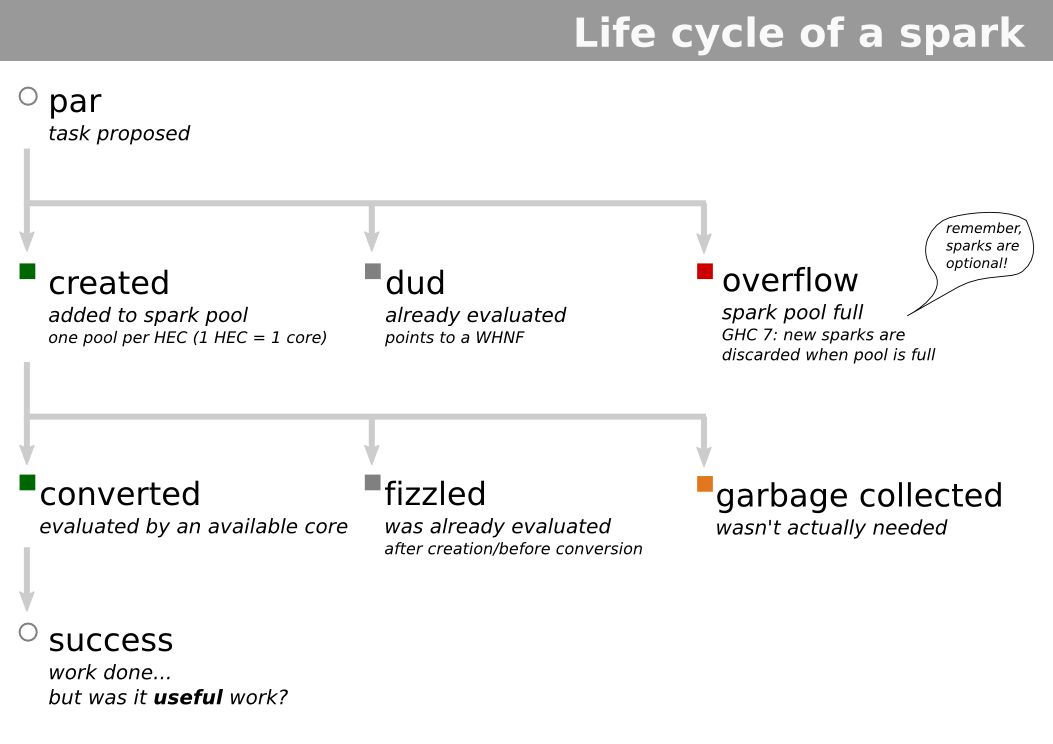
\includegraphics[width=0.8\textwidth]{Spark-lifecycle}}

  Der Lebenszyklus eines Sparks.
  Quelle: \url{https://wiki.haskell.org/ThreadScope_Tour/Spark}
\end{center}


\subsection{Threads}

Mit \haskellinline{forkIO :: IO a -> IO ThreadId} aus dem Modul
\haskellinline{Control.Concurrent} erzeugt man einen \emph{leichtgewichtigen
Thread}. Die übergebene IO-Aktion wird in diesem Thread ausgeführt;
Rückgabewert ist ein Wert vom Typ \haskellinline{ThreadId}, mit dem man den
Thread noch nachträglich kontrollieren (etwa vorzeitig beenden) kann.

Die Laufzeitumgebung kommt mit sehr vielen -- Millionen -- von
leichtgewichtigen Threads klar. Sie werden auf eine kleine Anzahl
echter Threads auf Betriebssystem-Level verteilt.

In speziellen Anwendungsfällen ist es nötig, Betriebssystem-Threads statt
leichtgewichtiger Threads zu erzeugen. Das ist mittels der Funktion
\haskellinline{forkOS :: IO a -> IO ThreadId} ebenfalls möglich.

\emph{Wichtig:} Wenn man Threads nur verwenden möchte, um mit simultan
stattfindenden IO-Aktionen umzugehen (etwa Anforderungen mehrerer gleichzeitig
verbundener Clients über das Netzwerk entgegennehmen), genügt prinzipiell ein
einzelner Betriebssystem-Thread. Wenn man aber mit Threads
tatsächlich auch mehrere Berechnungen parallel ausführen möchte, muss man
wie im vorherigen Abschnitt beschrieben seinen Code mit der Option
\texttt{-threaded} kompilieren und beim Ausführen
dem Laufzeitsystem mit \texttt{+RTS -N -RTS} mitteilen, mehrere
Betriebssystem-Threads zu verwenden.

\begin{aufgabe}{Hallo Welt aus zwei Threads}
Schreibe ein Haskell-Programm, das einen leichtgewichtigen Thread erzeugt
und den ausführenden Lambroiden sowohl vom Hauptthread als auch dem erzeugten
Thread mit \haskellinline{putStrLn} grüßt.
\end{aufgabe}

\begin{aufgabe}{Vermischte Ausgabe}
Schreibe ein Haskell-Programm, das zwei leichtgewichtige Threads erzeugt. Der
eine Thread soll tausendmal das Zeichen \haskellinline{'a'} ausgeben, der
andere das Zeichen \haskellinline{'b'}. Was passiert?
\end{aufgabe}

\begin{aufgabe}{Sleep Sort}
Implementiere \emph{Sleep Sort}: Erzeuge für jedes
Element~\haskellinline{x} einer gegebenen Liste von (kleinen) natürlichen
Zahlen einen Thread, der sich gleich nach seiner Erstellung für eine
zu~\haskellinline{x} proportionale Zeit schlafen legt und
anschließend~\haskellinline{x} auf dem Terminal ausgibt.

{\scriptsize\emph{Tipp.} Verwende die Funktion \haskellinline[fontsize=\scriptsize]{threadDelay ::
Int -> IO ()}, die den momentan laufenden Thread für eine gegebene Anzahl
Mikrosekunden schlafen legt.\par}
\end{aufgabe}

Eine primitive Möglichkeit der Kommunikation zwischen Threads sind
(thread-sichere) veränderliche Variablen. Eine solche kann zu jedem Zeitpunkt
leer sein oder einen Wert enthalten. Man erstellt sie mit
\haskellinline{newEmptyMVar :: IO (MVar a)} oder, wenn man die Variable gleich
initialiseren möchte, mit \haskellinline{newMVar :: a -> IO (MVar a)}.

Mit \haskellinline{readMVar :: MVar a -> IO a} holt man den aktuellen Wert
einer übergebenen Variable. Sollte die Variable leer sein, blockiert dieser
Aufruf so lange, bis die Variable durch einen anderen Thread gefüllt wird.

Eine Variante ist die Funktion \haskellinline{takeMVar :: MVar a -> IO a}, die
nach Auslesen der Variable diese leert.

Mit \haskellinline{putMVar :: MVar a -> a -> IO ()} setzt man den Inhalt einer
Variable. Wenn diese zum Zeitpunkt des Aufrufs nicht leer sein sollte, wird der
vorhandene Inhalt nicht überschrieben. Stattdessen wird der ausführende Thread
so schlafen gelegt, bis ein anderer Thread die Variable mit
\haskellinline{takeMVar} leert. (Es gibt auch \haskellinline{tryPutMVar :: MVar
-> a -> IO Bool}, das den Thread nicht schlafen geht und den Erfolg durch den
Rückgabewert anzeigt.)

\begin{aufgabe}{Lesen aus einer dauerhaft leeren Variable}
Was macht folgender Code? Wie reagiert das Laufzeitsystem von GHC?

\begin{haskellcode}
import Control.Concurrent

main = do
    ref <- newEmptyMVar
    takeMVar ref
\end{haskellcode}
\end{aufgabe}

\begin{aufgabe}{Ein einfaches Beispiel zu Variablen}
Schreibe ein Programm, das zwei leichtgewichtigen Threads erzeugt, die je eine große
Fibonacci-Zahl berechnen und das Ergebnis in je einer Variable speichern. Der
Hauptthread soll dann die beiden Ergebnisse ausgeben.
\end{aufgabe}

\begin{aufgabe}{Vorsicht vor Deadlocks}
Was macht folgender Code? Wie reagiert das Laufzeitsystem von GHC?

\begin{haskellcode}
import Control.Concurrent

main = do
    ref1 <- newEmptyMVar
    ref2 <- newEmptyMVar
    forkIO $ takeMVar ref2 >> putMVar ref1 "Hallo Welt"
    putStrLn =<< takeMVar ref1
\end{haskellcode}
\end{aufgabe}

\begin{aufgabe}{Warten auf Kinder}
Oft möchte man im Hauptthread die Beendigung gestarteter Threads abwarten. Das
ist zum Beispiel mit folgendem Code möglich (den es natürlich auch schon in
verpackter Form im Modul \textinline{Control.Concurrent.Async} gibt).
Vollziehe ihn nach!

\begin{haskellcode}
import Control.Monad
import Control.Concurrent

forkThread :: IO () -> IO (MVar ())
forkThread proc = do
    ref <- newEmptyMVar
    forkFinally proc $ \_ -> putMVar ref ()
    return ref

main = do
    jobs <- mapM forkThread [...]
    mapM_ takeMVar jobs
\end{haskellcode}
\end{aufgabe}

Neben veränderlichen Variablen gibt es noch \emph{Kanäle} zur Kommunikation
zwischen Threads. Kanäle können anders als Variablen mehr als einen Wert
zwischenspeichern. Man erzeugt einen Kanal mit \haskellinline{newChan :: IO
(Chan a)}, pusht einen Wert durch \haskellinline{writeChan :: Chan a -> a ->
IO ()} und poppt den vordersten Wert mit \haskellinline{readChan :: Chan a ->
IO a}. Der Aufruf von \haskellinline{readChan} blockiert, falls der Kanal leer
ist.

\begin{aufgabe}{Sleep Sort kanalbasiert}
Modifiziere deinen Sleep-Sort-Algorithmus derart, dass die sortierten Werte
nicht auf dem Terminal ausgegeben, sondern in einen Kanal geschrieben werden.
Dieser soll dann in einem Rutsch ausgegeben werden. 
\end{aufgabe}

Zum Ende dieses Abschnitts sei bemerkt, dass man selten auf der Ebene dieser
Aufgaben programmieren muss. Für viele Einsatzgebiete gibt es schon fertige
Kombinatoren-Bibliotheken zum nebenläufigen Programmieren.

\begin{aufgabe}{Projekt: Ein einfacher Chat-Server}
Vervollständige folgende Vorlage für einen einfachen Chat-Server. Clients
sollen sich mit ihm auf TCP-Port~4242 verbinden können. Eingehende Nachrichten
sollen an alle verbundenen Clients weitergeleitet werden.

Diese Vorlage ist auf einem niedrigen Level, mit expliziten Socket-Operationen,
geschrieben. Normalerweise würde man eine High-Level-Streaming-Bibliothek wie
Conduits oder Pipes verwenden. Diese kümmern sich auch automatisch um
ordnungsgemäßes Abmelden von Clients.

{\scriptsize\emph{Tipp.} Verwende die Funktion \haskellinline{dupChan :: Chan a
-> IO (Chan a)}. \emph{Bonusaufgabe.} Identifiziere das Speicherleckproblem und
löse es.\par}

\begin{haskellcode}
module Main where

import Control.Monad
import Control.Concurrent
import Network.Socket
import System.IO

main :: IO ()
main = do
    -- Lausche auf Port 4242.
    sock <- socket AF_INET Stream 0
    setSocketOption sock ReuseAddr 1
    bindSocket sock (SockAddrInet 4242 iNADDR_ANY)
    listen sock 10

    -- Setze einen Kanal auf. Was in diesen Kanal geschrieben wird,
    -- soll an alle verbundenen Clients weitergeleitet werden.
    ...

    -- Die Hauptschleife: Akzeptiere laufend neue Verbindungen und
    -- bearbeite sie.
    forever $ do
        (conn,_) <- accept sock
        hdl      <- socketToHandle conn ReadWriteMode
        hSetBuffering hdl NoBuffering
        -- `hdl` ist nun ein gewöhnlicher Handle, mit dem `hGetLine`
        -- und `hPutStrLn` verwendet werden können.

        -- Dupliziere den Kanal, um mehrere Zuhörer zu unterstützen.
        ...

        -- Schreibe gelesene Nachrichten in den Kanal.
        forkIO $ forever $ do
            msg <- hGetLine hdl
            ...

        -- Leite Nachrichten der anderen Verbindungen weiter.
        forkIO $ forever $ do
            ...
            hPutStrLn hdl msg
\end{haskellcode}
\end{aufgabe}


\subsection{Shared Transactional Memory (STM)}

In dem folgenden Programm kommt es zu einer Race Condition. Wiederholte Aufrufe
des Programms werden verschiedene Ergebnisse liefern.

\begin{haskellcode}
import Control.Concurrent
import Control.Monad

forkThread :: IO () -> IO (MVar ())
forkThread = {- siehe oben -}

go :: IORef Integer -> IORef Integer -> IO ()
go xRef yRef = do
    x <- readIORef xRef
    y <- readIORef yRef
    let x' = y  + 1
        y' = x' + 1
    writeIORef xRef x'
    writeIORef yRef y'

main = do
    xRef <- newIORef 1
    yRef <- newIORef 2
    jobs <- replicateM 40000 $ forkThread $ go xRef yRef
    mapM_ takeMVar jobs
    x <- readIORef xRef
    y <- readIORef yRef
    print (x, y)
\end{haskellcode}

Mit STM passiert das nicht. Statt \haskellinline{IORef}'s verwendet man dann
\haskellinline{TVar}'s. Die Operationen übertragen sich wörtlich, spielen sich
dann aber in der \haskellinline{STM}- statt der \haskellinline{IO}-Monade ab:
\haskellinline{newTVar :: a -> STM (TVar a)} und so weiter. Man führt
STM-Aktionen mit \haskellinline{atomically :: STM a -> IO a} aus.

Der angepasste Code sieht so aus:

\begin{haskellcode}
import Control.Concurrent
import Control.Concurrent.STM
import Control.Monad

forkThread :: IO () -> IO (MVar ())
forkThread = {- siehe oben -}

go :: TVar Integer -> TVar Integer -> STM ()
go xRef yRef = do
    x <- readTVar xRef
    y <- readTVar yRef
    let x' = y  + 2
        y' = x' + 2
    writeTVar xRef x'
    writeTVar yRef y'

main = do
    xRef <- newTVarIO 1
    yRef <- newTVarIO 2
    jobs <- replicateM 40000 $ forkThread $ atomically $ go xRef yRef
    mapM_ takeMVar jobs
    x <- readTVarIO xRef
    y <- readTVarIO yRef
    print (x, y)
\end{haskellcode}

Wie funktioniert STM? In erster Näherung so: Wird ein
\haskellinline{atomically}-Block ausgeführt, so werden Änderungen an
\haskellinline{TVar}'s nicht sofort geschrieben. Stattdessen werden sie in
einem Log notiert. Am Ende des Blocks prüft das Laufzeitsystem in einer
atomaren Operation, ob sich seit Ablauf des Blocks seine Abhängigkeiten (zum
Beispiel veränderliche Variablen, auf die lesend zugegriffen wurde) geändert
haben. Wenn nein, macht es die Änderungen an den \haskellinline{TVar}'s
wirksam. Wenn ja, wird der Block einfach erneut ausgeführt. Da in der
STM-Monade nicht beliebige Nebenwirkungen wie \haskellinline{fireMissiles}
möglich sind, ist das ein fundiertes Vorgehen.

\end{document}

XXX: Ein paar Aufgaben zu `par` und `pseq` verfassen.
